\documentclass[tikz, border=14pt]{standalone}
\usepackage{amsmath}
\usepackage{amssymb}
\usepackage{tikz}
\usetikzlibrary{positioning, arrows.meta, calc, fit, backgrounds}

% ── Palette ─────────────────────────────────────────────────────────────────
\definecolor{cFlow}   {RGB}{219,234,254}
\definecolor{cScore}  {RGB}{254,243,199}
\definecolor{cState}  {RGB}{204,251,241}
\definecolor{cActor}  {RGB}{237,233,254}
\definecolor{cAction} {RGB}{252,231,243}
\definecolor{cReward} {RGB}{220,252,231}
\definecolor{cCritic} {RGB}{254,226,226}
\definecolor{cBorder} {RGB}{ 71, 85,105}
\definecolor{cLag}    {RGB}{185, 28, 28}

\begin{document}
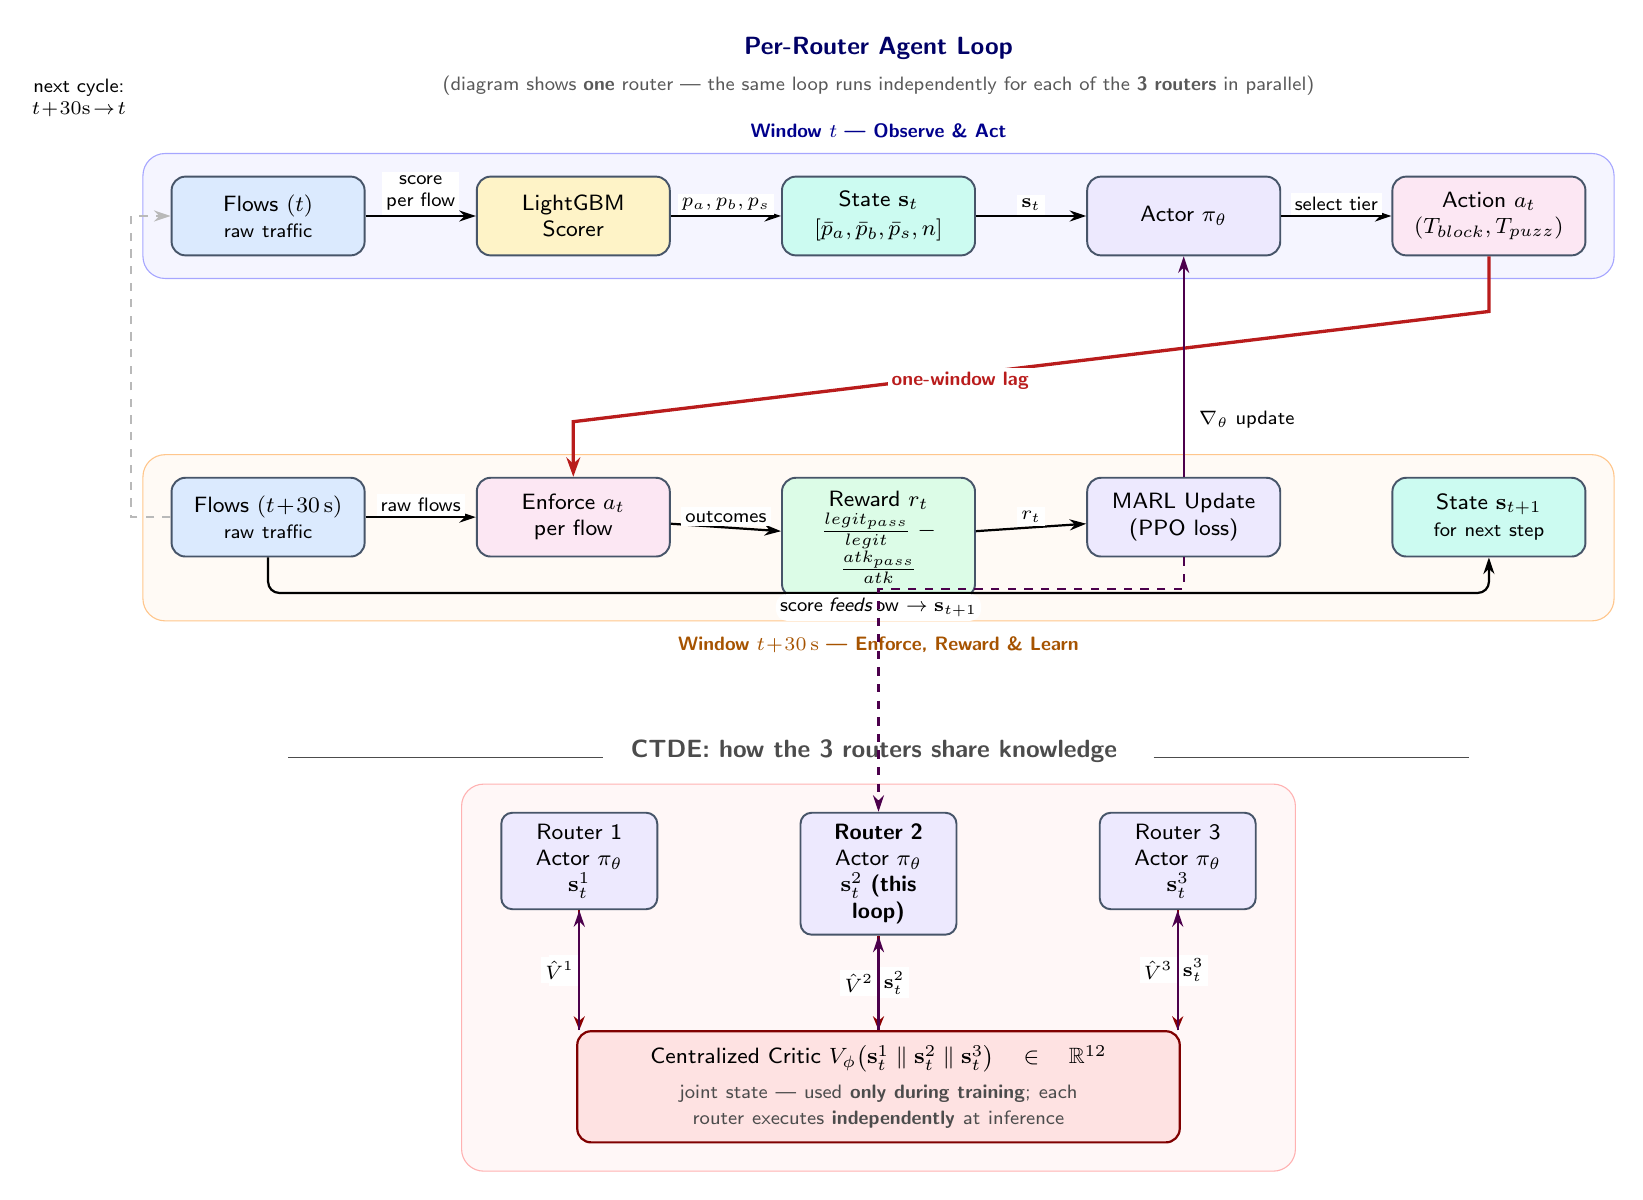
\begin{tikzpicture}[
  font=\sffamily\footnotesize,
  %──── node styles ────────────────────────────────────────────────────────
  box/.style={
    draw=cBorder, rounded corners=5pt, line width=0.7pt,
    minimum width=2.3cm, minimum height=1.0cm,
    align=center, text width=2.1cm, inner sep=5pt
  },
  flows/.style  = {box, fill=cFlow},
  scorer/.style = {box, fill=cScore},
  stateb/.style = {box, fill=cState},
  actor/.style  = {box, fill=cActor},
  action/.style = {box, fill=cAction},
  reward/.style = {box, fill=cReward},
  critic/.style = {box, fill=cCritic},
  miniactor/.style = {
    draw=cBorder, rounded corners=4pt, line width=0.7pt,
    minimum width=1.9cm, minimum height=0.85cm,
    align=center, text width=1.7cm, inner sep=4pt, fill=cActor
  },
  %──── arrow styles ───────────────────────────────────────────────────────
  arr/.style     = {-{Stealth[length=6pt,width=4pt]}, thick, black},
  lag/.style     = {-{Stealth[length=7pt,width=5pt]}, very thick, cLag},
  policy/.style  = {-{Stealth[length=6pt,width=4pt]}, thick, draw=violet!60!black},
  feedback/.style= {-{Stealth[length=6pt,width=4pt]}, thick, draw=gray!55, dashed},
  ctdearr/.style = {-{Stealth[length=5pt,width=4pt]}, thick, draw=red!55!black},
  lbl/.style     = {font=\scriptsize\sffamily, fill=white, inner sep=1.5pt, midway, align=center},
]

%% ════════════════════════════════════════════════════════════════════════
%%  ROW 1 — Window t  (OBSERVE + ACT)
%% ════════════════════════════════════════════════════════════════════════
\node[flows]  (Wt)  {Flows $(t)$\\{\scriptsize raw traffic}};
\node[scorer, right=1.4cm of Wt]  (Lt)
  {LightGBM\\Scorer};
\node[stateb, right=1.4cm of Lt]  (St)
  {State $\mathbf{s}_t$\\[1pt]$[\bar{p}_{a},\bar{p}_{b},\bar{p}_{s},n]$};
\node[actor,  right=1.4cm of St]  (A)
  {Actor $\pi_\theta$};
\node[action, right=1.4cm of A]   (at)
  {Action $a_t$\\$(T_{block},T_{puzz})$};

%% ════════════════════════════════════════════════════════════════════════
%%  ROW 2 — Window t+1  (ENFORCE + OBSERVE again + LEARN)
%% ════════════════════════════════════════════════════════════════════════
\node[flows,  below=2.8cm of Wt]  (Wt1)
  {Flows $(t\!+\!30\,\mathrm{s})$\\{\scriptsize raw traffic}};
\node[action, below=2.8cm of Lt]  (Enf)
  {Enforce $a_t$\\per flow};
\node[reward, below=2.8cm of St]  (Rt)
  {Reward $r_t$\\$\tfrac{legit_{pass}}{legit} - \tfrac{atk_{pass}}{atk}$};
\node[actor,  below=2.8cm of A]   (M)
  {MARL Update\\(PPO loss)};
\node[stateb, below=2.8cm of at]  (St1)
  {State $\mathbf{s}_{t+1}$\\{\scriptsize for next step}};

%% ════════════════════════════════════════════════════════════════════════
%%  TITLE  (above row 1, centered)
%% ════════════════════════════════════════════════════════════════════════
\node[above=0.9cm of $(Wt.north)!0.5!(at.north)$,
      font=\sffamily\small\bfseries, text=blue!40!black,
      align=center] (title)
  {Per-Router Agent Loop\\[2pt]
   {\normalfont\scriptsize\sffamily\color{gray!70!black}%
    (diagram shows \textbf{one} router — the same loop runs independently
    for each of the \textbf{3 routers} in parallel)}};

%% ════════════════════════════════════════════════════════════════════════
%%  ARROWS — ROW 1
%% ════════════════════════════════════════════════════════════════════════
\draw[arr] (Wt) -- node[lbl,above]{score\\per flow} (Lt);
\draw[arr] (Lt) -- node[lbl,above]{$p_a,p_b,p_s$} (St);
\draw[arr] (St) -- node[lbl,above]{$\mathbf{s}_t$} (A);
\draw[arr] (A)  -- node[lbl,above]{select tier} (at);

%% ════════════════════════════════════════════════════════════════════════
%%  ONE-WINDOW LAG
%% ════════════════════════════════════════════════════════════════════════
\draw[lag]
  (at.south) -- ++(0,-0.7)
  -- node[lbl, below, xshift=-0.9cm]
     {\textbf{\color{cLag}one-window lag}}
  ($(Enf.north)+(0,0.7)$)
  -- (Enf.north);

%% ════════════════════════════════════════════════════════════════════════
%%  ARROWS — ROW 2
%% ════════════════════════════════════════════════════════════════════════
\draw[arr] (Wt1.east)  -- node[lbl,above]{raw flows}   (Enf.west);
\draw[arr] (Enf)       -- node[lbl,above]{outcomes}    (Rt);
\draw[arr] (Rt)        -- node[lbl,above]{$r_t$}       (M);
\draw[arr, rounded corners=4pt]
  (Wt1.south) -- ++(0,-0.45)
  -- node[lbl,below]{score per flow $\to\mathbf{s}_{t+1}$}
  ($(St1.south)+(0,-0.45)$)
  -- (St1.south);

%% ════════════════════════════════════════════════════════════════════════
%%  POLICY UPDATE
%% ════════════════════════════════════════════════════════════════════════
\draw[policy]
  (M.north) -- ++(0,0.55) -|
  node[lbl, above, xshift=0.8cm]{$\nabla_\theta$ update}
  (A.south);

%% ════════════════════════════════════════════════════════════════════════
%%  FEEDBACK — Flows t+1 → t
%% ════════════════════════════════════════════════════════════════════════
\draw[feedback]
  (Wt1.west) -- ++(-0.5,0)
  |- node[lbl, left, yshift=1.5cm]{next cycle:\\$t\!+\!30\mathrm{s}\!\to\!t$}
  (Wt.west);

%% ════════════════════════════════════════════════════════════════════════
%%  CTDE PANEL  — 3 routers + shared centralized critic
%% ════════════════════════════════════════════════════════════════════════

%% Separator label
\node[below=2.2cm of $(Wt1.south)!0.5!(St1.south)$,
      font=\sffamily\bfseries\small, text=gray!60!black] (sep)
  {\rule{4cm}{0.4pt}\quad CTDE: how the 3 routers share knowledge \quad\rule{4cm}{0.4pt}};

%% Three mini actor nodes
\node[miniactor, below=0.5cm of sep, xshift=-3.8cm] (R1)
  {Router 1\\Actor $\pi_\theta$\\$\mathbf{s}^1_t$};
\node[miniactor, below=0.5cm of sep] (R2)
  {\textbf{Router 2}\\Actor $\pi_\theta$\\$\mathbf{s}^2_t$ \textbf{(this loop)}};
\node[miniactor, below=0.5cm of sep, xshift=3.8cm] (R3)
  {Router 3\\Actor $\pi_\theta$\\$\mathbf{s}^3_t$};

%% Shared centralized critic
\node[critic,
      draw=red!50!black, line width=0.8pt,
      minimum width=7.5cm, text width=7.3cm,
      minimum height=1.1cm,
      below=1.2cm of R2] (CC)
  {Centralized Critic $V_\phi\!\left(\mathbf{s}^1_t \;\|\; \mathbf{s}^2_t \;\|\; \mathbf{s}^3_t\right)
   \;\in\; \mathbb{R}^{12}$\\[3pt]
   {\scriptsize\color{gray!60!black}
   joint state — used \textbf{only during training};
   each router executes \textbf{independently} at inference}};

%% Arrows: actors → critic (states)
\draw[ctdearr] (R1.south) -- node[lbl,left] {$\mathbf{s}^1_t$} (R1.south|-CC.north);
\draw[ctdearr] (R2.south) -- node[lbl,right]{$\mathbf{s}^2_t$} (R2.south|-CC.north);
\draw[ctdearr] (R3.south) -- node[lbl,right]{$\mathbf{s}^3_t$} (R3.south|-CC.north);

%% Arrows: critic → actors (value estimates / gradients)
\draw[policy] (CC.north-|R1) -- node[lbl,left] {$\hat{V}^1$} (R1.south);
\draw[policy] (CC.north-|R2) -- node[lbl,left] {$\hat{V}^2$} (R2.south);
\draw[policy] (CC.north-|R3) -- node[lbl,left] {$\hat{V}^3$} (R3.south);


%% Link: MARL Update in main diagram → shared critic concept
\draw[policy, dashed]
  (M.south) -- ++(0,-0.4)
  -| node[lbl, left, yshift=-0.2cm]{\textit{feeds}} (R2.north);

%% ════════════════════════════════════════════════════════════════════════
%%  PHASE BACKGROUND BOXES
%% ════════════════════════════════════════════════════════════════════════
\begin{scope}[on background layer]
  %% Window t
  \node[draw=blue!35, fill=blue!4, rounded corners=8pt,
        inner xsep=10pt, inner ysep=8pt,
        fit=(Wt)(Lt)(St)(A)(at),
        label={[font=\scriptsize\sffamily\bfseries, text=blue!55!black,
                yshift=2pt]above:Window $t$ — \textsc{Observe \& Act}}] {};
  %% Window t+1
  \node[draw=orange!45, fill=orange!4, rounded corners=8pt,
        inner xsep=10pt, inner ysep=8pt,
        fit=(Wt1)(Enf)(Rt)(M)(St1),
        label={[font=\scriptsize\sffamily\bfseries, text=orange!65!black,
                yshift=-2pt]below:Window $t\!+\!30\,\mathrm{s}$ — \textsc{Enforce, Reward \& Learn}}] {};
  %% CTDE panel
  \node[draw=red!30, fill=red!3, rounded corners=8pt,
        inner xsep=14pt, inner ysep=10pt,
        fit=(R1)(R2)(R3)(CC)] {};
\end{scope}

\end{tikzpicture}
\end{document}
